\documentclass[12]{beamer}
\usepackage{multicol}
\usepackage{enumitem}
\usepackage{listings}
\lstnewenvironment{python}{\lstset{language=python}}{}
\lstnewenvironment{java}{\lstset{style=customjava,language=java}}{}

\lstdefinestyle{customjava}{
  belowcaptionskip=1\baselineskip,
  breaklines=true,
  language=java,
  showstringspaces=false,
  basicstyle=\footnotesize\ttfamily,
  keywordstyle=\bfseries\color{green!40!black},
  commentstyle=\itshape\color{purple!40!black},
  identifierstyle=\color{blue},
  stringstyle=\color{orange},
  escapeinside={(*@}{@*)},
  tabsize=4
}

\usetheme[progressbar=frametitle]{metropolis}
\setbeamertemplate{frame numbering}[fraction]
\usefonttheme{metropolis}
\usecolortheme{spruce}
\setbeamercolor{background canvas}{bg=white}
\setbeamercovered{transparent=5}
\metroset{block=fill}

\definecolor{mygreen}{rgb}{125, 5, 25}
\usecolortheme[named=mygreen]{structure}



\title{Week 11 Practical}
\author{Brae}
\institute {CSSE2002: Programming in the Large}

\begin{document}

\begin{frame}
\titlepage
\end{frame}

\begin{frame}[t, fragile]{This Week in CSSE2002} \vspace{4pt}

This week we will begin looking at javafx, the practical sheet and associated material assist you to write three gui interfaces.

\begin{onlyenv}<2->
\textbf{Note: Supplied code not required until third interface}
\end{onlyenv}

\begin{onlyenv}<3->

\begin{columns}[onlytextwidth]
\column{0.4\textwidth}
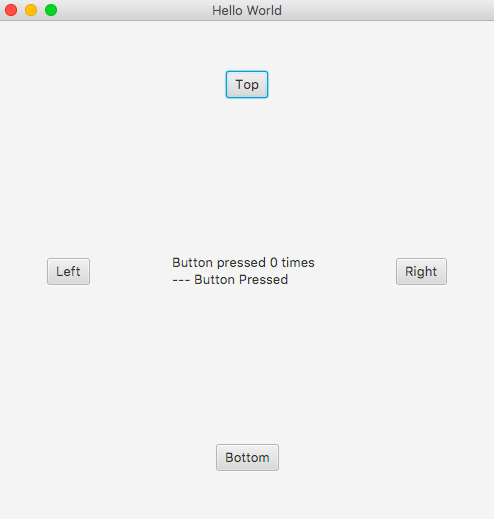
\includegraphics[scale=0.25]{resources/week11prac1}\\[20pt]
\column{0.6\textwidth}
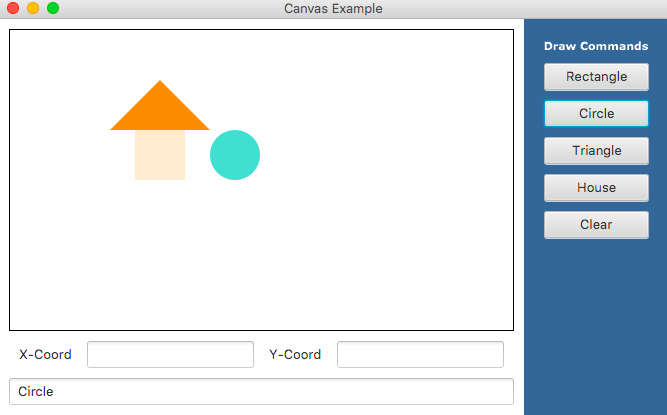
\includegraphics[scale=0.25]{resources/week11prac2}\\[20pt]
\end{columns}

\end{onlyenv}

\end{frame}

\end{document}
